\documentclass[11pt,letterpaper]{article}

\usepackage[utf8]{inputenc}
\usepackage[T1]{fontenc}
\usepackage{microtype}

% Page layout
\usepackage[letterpaper,top=1in,bottom=2cm,left=1in,right=1in]{geometry}

% Par skip
\usepackage[skip=5pt plus 3pt minus 1pt,parfill=0pt]{parskip}
% the code below fixed the spacing before theorems.
\makeatletter
\def\thm@space@setup{%
  \thm@preskip=\parskip \thm@postskip=0pt
}
% Run-in paragraph headings get only the usual \parskip above them
% (parskip subtracts \parskip from the space before a heading).
\renewcommand\paragraph{\@startsection{paragraph}{4}{\z@}{\parskip}{-1em}{\normalfont\normalsize\bfseries}}
\makeatother


% Math and theorems
\usepackage{amsmath}
\usepackage{amsthm}
\usepackage{thm-restate}
\usepackage{mathtools}

% Special fonts and symbols
\usepackage{amssymb}
\usepackage{bm,dsfont}
\usepackage{csquotes}
\usepackage{nicefrac}

% Colors
\usepackage{xcolor}

\definecolor{col1}{HTML}{56b3e9}
\definecolor{col2}{HTML}{e69f00}
\definecolor{col3}{HTML}{009e74}
\definecolor{col4}{HTML}{cc79a7}
\definecolor{col5}{HTML}{d55e00}
\definecolor{col6}{HTML}{0071b2}

% Figures
\usepackage[small]{caption}
\usepackage{subcaption}
\usepackage{tikz}
\usepackage{pgfplots}
\pgfplotsset{compat=1.18}

% Tables
\usepackage{booktabs}
\usepackage{array}

% Enumerations
\usepackage[shortlabels]{enumitem}

% Appendix
\usepackage[toc,page]{appendix}

% Citations
\usepackage[
 backend=biber,
 style=alphabetic,
 citetracker,
 hyperref=auto,
 maxcitenames=10,
 minalphanames=3,
 maxalphanames=4,
 sortcites,
 sorting=nyt,
 maxbibnames=12,
 date=year,
 isbn=false,
 url=false,
 doi=false,
 eprint=false,
]{biblatex}
\addbibresource{literature.bib}

\newbibmacro{string+doiurl}[1]{%
  \iffieldundef{doi}{%
    \iffieldundef{url}{%
      #1
    }{%
      \href{\thefield{url}}{#1}%
    }%
  }{%
    \href{http://dx.doi.org/\thefield{doi}}{#1}%
  }%
}

\AtEveryCitekey{%
  \ifciteseen
    {\defcounter{maxnames}{2}}
    {}%
}

\DeclareFieldFormat%
[article,inbook,incollection,inproceedings,patent,thesis,unpublished]
  {title}{\usebibmacro{string+doiurl}{#1}}

% References and hyperlinks
\usepackage[colorlinks]{hyperref}
\hypersetup{citecolor=green!60!black,linkcolor=blue!70!black,urlcolor=blue!70!black}
\usepackage[capitalize, noabbrev, nameinlink]{cleveref}
\crefname{condition}{condition}{conditions}
\Crefname{condition}{Condition}{Conditions}
\usepackage{xurl}
\hypersetup{breaklinks=true}

% Auxiliary packages
\usepackage{xspace}

\allowdisplaybreaks

\newtheorem{theorem}{Theorem}[section]
\newtheorem{lemma}[theorem]{Lemma}
\newtheorem{claim}[theorem]{Claim}
\newtheorem{fact}[theorem]{Fact}
\newtheorem{corollary}[theorem]{Corollary}
\newtheorem{proposition}[theorem]{Proposition}
\newtheorem{observation}[theorem]{Observation}

\theoremstyle{definition}
\newtheorem{definition}[theorem]{Definition}
\newtheorem{example}[theorem]{Example}

\theoremstyle{remark}
\newtheorem{remark}[theorem]{Remark}


% General math stuff
\DeclarePairedDelimiter\ceil{\lceil}{\rceil}
\DeclarePairedDelimiter\floor{\lfloor}{\rfloor}
\DeclarePairedDelimiter{\abs}{\lvert}{\rvert}
\DeclarePairedDelimiter{\scp}{\langle}{\rangle}
\DeclareMathOperator*{\argmax}{arg\,max}
\DeclareMathOperator*{\argmin}{arg\,min}
\newcommand{\supp}{\mathrm{supp}}

\newcommand{\RR}{\mathbb{R}}
\newcommand{\NN}{\mathbb{N}}
\newcommand{\bone}{\mathbf{1}}
\newcommand{\dd}{\,\mathrm{d}}

% Problems and algorithms
\newcommand{\psp}{\relax\ifmmode{\mathrm{PSP}}\else PSP\xspace\fi}
\newcommand{\ALG}{{\mathrm{ALG}}}
\newcommand{\OPT}{{\mathrm{OPT}}}
\newcommand{\PF}{\mathrm{PF}}
\newcommand{\CPA}{\mathrm{CPA}}
\newcommand{\LAPS}{\mathrm{LAPS}}
\newcommand{\WRR}{\mathrm{WRR}}
\newcommand{\LP}{\mathrm{LP}}
\newcommand{\DLP}{\mathrm{DLP}}

% Notation for input
\newcommand{\cP}{\mathcal{P}}
\newcommand{\cQ}{\mathcal{Q}}
\newcommand{\eps}{\varepsilon}

\usepackage[colorinlistoftodos,prependcaption,textsize=scriptsize]{todonotes}

\newcommand{\alexinline}[1]{\todo[linecolor=orange,backgroundcolor=orange!25,bordercolor=orange,inline]{A:~#1}}
\newcommand{\alex}[1]{\todo[linecolor=orange,backgroundcolor=orange!25,bordercolor=orange]{A:~#1}}
\newcommand{\sven}[1]{\todo[linecolor=green,backgroundcolor=green!25,bordercolor=green]{S:~#1}}
\newcommand{\sveninline}[1]{\todo[linecolor=green,backgroundcolor=green!25,bordercolor=green,inline]{S:~#1}}
\newcommand{\bart}[1]{\todo[linecolor=blue,backgroundcolor=blue!25,bordercolor=blue]{B:~#1}}
\newcommand{\bartinline}[1]{\todo[linecolor=blue,backgroundcolor=blue!25,bordercolor=blue,inline]{B:~#1}}


% Additions for this paper
\usetikzlibrary{decorations.pathreplacing}
\newcommand{\E}{\mathbb{E}}
\newcommand{\cD}{\mathcal{D}}
\newcommand{\cA}{\mathcal{A}}
\newcommand{\cF}{\mathcal{F}}
\newcommand{\Amp}{\mathrm{Amp}}
\newcommand{\Avg}{\mathrm{Avg}}


\sloppy

\title{Weighted Flow Time Does Not Admit\\ $O(1)$-Competitive Randomized Algorithms}

\author{%
}
\date{}

\begin{document}

\maketitle

\begin{abstract}
We study the classical online problem of scheduling jobs with release times, sizes, and weights on a single machine with preemption so as to minimize the total weighted flow time. Bansal and Chan (SODA~2009) showed that no deterministic online algorithm is $O(1)$-competitive for this problem. We show that randomization does not overcome this barrier: no randomized online algorithm is $O(1)$-competitive against an oblivious adversary. Quantitatively, every randomized algorithm has competitive ratio $\Omega(\min\{\log\log W,\log\log\log P\})$, where $W$ and $P$ are the ratios between the largest and the smallest weight and size, respectively.

Following Yao's principle, we construct a single distribution over instances that defeats every deterministic algorithm. The construction compares the unfinished weight of the algorithm with that of an optimal schedule at a random terminal time that the algorithm cannot observe, and it alternates two operations. Amplification appends a heavy job and draws the terminal time from a geometric distribution, so that the algorithm has to leave either the heavy job or its earlier backlog unfinished. Averaging concatenates independent copies at decreasing time scales and uses martingale concentration to make the backlog of the algorithm almost deterministic, which allows us to amplify again.
\end{abstract}

\section{Introduction}

We consider one of the most basic problems in online scheduling: jobs arrive over time at a single machine, and the goal is to minimize their total weighted flow time. Each job~$j$ has a release time~$r_j$, a size~$p_j$, and a weight~$w_j$, which become known at time~$r_j$. The machine processes at most one job at a time, and a job may be preempted and resumed later. If job~$j$ completes at time~$C_j$, its flow time is $C_j-r_j$, and the objective is to minimize $\sum_j w_j(C_j-r_j)$. An online algorithm decides at every time which job to process, without knowledge of future jobs. It is \emph{$R$-competitive} if, on every instance, its (expected) cost is at most $R$ times the optimal cost, up to an additive constant.

For unit weights, always processing the job with the shortest remaining processing time is optimal~\cite{Schrage68}. With weights, the problem is considerably harder. Already the offline problem is strongly NP-hard~\cite{LabetoulleLLR84}, and a polynomial-time approximation scheme was found only recently~\cite{ArmbrusterRW23}, after a long line of work~\cite{ChekuriK02,BansalP10,BatraGK18,FeigeKL19,RohwedderW21}. In the online setting, the first algorithm with a nontrivial competitive ratio is due to Chekuri, Khanna, and Zhu~\cite{ChekuriKZ01}; it is semi-online, as it needs to know~$P$ in advance, and $O(\log^2 P)$-competitive, where $P$ is the ratio between the largest and the smallest job size. Bansal and Dhamdhere~\cite{BansalD07} gave an $O(\log W)$-competitive algorithm, where $W$ is the ratio between the largest and the smallest weight. Azar and Touitou~\cite{AzarT18} gave an $O(\log P)$-competitive and an $O(\log D)$-competitive algorithm, where $D$ is the ratio between the largest and the smallest density $w_j/p_j$, and combined these results with the algorithm of Bansal and Dhamdhere into an $O(\log\min\{P,D,W\})$-competitive algorithm. On a machine that is faster by a factor of $1+\eps$, the simple Highest Density First rule is $O(1/\eps)$-competitive~\cite{BecchettiLMP01}.

It was widely believed that weighted flow time admits an $O(1)$-competitive online algorithm, until Bansal and Chan~\cite{BansalC09} showed that every deterministic online algorithm has competitive ratio
\[
  \Omega\biggl(\min\biggl\{\sqrt{\frac{\log W}{\log\log W}},\,\sqrt{\frac{\log\log P}{\log\log\log P}}\biggr\}\biggr).
\]
Their proof introduced a gap amplification technique: starting from the trivial lower bound of one, the lower bound is improved step by step, while the instance grows only moderately. Their adversary constructs the instance depending on the decisions of the algorithm, as is common for lower bounds against deterministic algorithms, and such an argument does not apply to randomized algorithms.

Randomization can be very powerful for flow time. For instance, if job sizes are unknown until the jobs complete, every deterministic algorithm for unweighted flow time on a single machine has competitive ratio $\Omega(n^{1/3})$, where $n$ is the number of jobs~\cite{MotwaniPT94}, while a randomized version of the multilevel feedback algorithm~\cite{KalyanasundaramP03} is $O(\log n)$-competitive~\cite{BecchettiL04}, which is best possible~\cite{MotwaniPT94}. For weighted flow time on a single machine, the only lower bound for randomized algorithms that we are aware of is the constant~$4/3$ of Chekuri, Khanna, and Zhu~\cite{ChekuriKZ01}. Thus, it has remained open whether a randomized online algorithm can be $O(1)$-competitive for weighted flow time.

\paragraph{Our results.}
We show that this is not the case.

\begin{theorem}\label{thm:main}
No randomized online algorithm for minimizing the total weighted flow time on a single machine is $O(1)$-competitive against an oblivious adversary. More precisely, for all $R\ge1$ and $\gamma\ge0$, there is a probability distribution~$\cD$ over finitely many instances such that every deterministic online algorithm~$A$ satisfies
\[
  \E_{I\sim\cD}\bigl[F_A(I)\bigr]\ge R\cdot\E_{I\sim\cD}\bigl[\OPT(I)\bigr]+\gamma.
\]
\end{theorem}

Here $F_A(I)$ denotes the weighted flow time of the schedule that $A$ produces on the instance~$I$, and $\OPT(I)$ is the optimal weighted flow time of~$I$. By Yao's principle, the second statement implies the first; the term~$\gamma$ rules out additive constants. The lower bound holds in a strong form: the algorithm learns the size and the weight of every job at its release, it may share the machine among several jobs, and it may know the distribution~$\cD$ in advance; in particular, it may know the number of jobs, which is the same for all instances of~$\cD$, and upper bounds on~$P$ and~$W$.

Our construction also gives an explicit, if weak, dependence on~$W$ and~$P$.

\begin{theorem}\label{thm:quant}
Every randomized online algorithm for weighted flow time has competitive ratio
\[
  \Omega\bigl(\min\{\log\log W,\,\log\log\log P\}\bigr)
\]
against an oblivious adversary on instances in which the ratios between the largest and the smallest weight and size are at most~$W$ and~$P$, respectively.
\end{theorem}

This dependence on $W$ and $P$ is exponentially weaker than in the deterministic lower bound of Bansal and Chan. It stems from the small improvement of each amplification step in our construction; see \cref{sec:conclusion}.

\subsection{Technical overview}\label{sec:overview}

By Yao's principle, it suffices to construct, for every~$R$, one distribution over instances on which every deterministic algorithm is worse than $R$ times the optimum in expectation. The difficulty compared with deterministic lower bounds is that the instance cannot react to the algorithm: the adversary does not know which jobs the algorithm has left unfinished. Instead, our distributions hide from the algorithm the time at which it is evaluated.

\paragraph{Gaps at a hidden terminal time.}
The building blocks of our construction are \emph{terminal distributions}: distributions over pairs $(I,T)$ of an instance~$I$ and a \emph{terminal time}~$T$ after all release times of~$I$. The algorithm processes~$I$ without knowing~$T$, and at time~$T$ we compare two quantities. On the offline side, $U^*(I,T)$ is the minimum weight that any schedule leaves unfinished at time~$T$. On the online side, we take the jobs that the algorithm leaves unfinished with remaining size at least~$1$, its \emph{robust backlog}, and we cap their total weight at a parameter~$M$. A terminal distribution is \emph{$(c,M)$-hard} if $\E[U^*(I,T)]\le1$, while every deterministic algorithm has an expected capped robust backlog of at least~$c$ (\cref{def:hard}). In words, at a moment that it cannot foresee, the algorithm has left $c$ times more weight unfinished than necessary, in jobs that it cannot complete quickly.

\paragraph{From a gap at one time to a gap in flow time.}
A $(2R,M)$-hard terminal distribution yields the lower bound~$R$. At the terminal time~$T$, we start a long stream of small jobs: every $d=1/(2M)$ time units, a job of size~$d$ and weight~$1/2$ arrives. The stream alone keeps the machine busy, so every unit of time that the algorithm spends on earlier jobs leaves one unit of stream volume unfinished, which has weight~$M$. To shrink its robust backlog, the algorithm must spend at least one unit of time on it, so its unfinished weight never drops below its capped robust backlog while the stream lasts. An optimal schedule, in contrast, may keep its unfinished weight $U^*(I,T)$ and process every stream job immediately, which costs $1/2$ per unit of time. For a long stream, the expected costs therefore differ by a factor of almost $2R/(1+1/2)>R$ (\cref{lem:flooding}). Thus it suffices to construct $(c,M)$-hard terminal distributions with arbitrarily large~$c$. We start from the trivial $(1,M)$-hard distribution that consists of a single job of size~$2$ with terminal time~$1$.

\paragraph{Copies at decreasing time scales.}
Both of our operations combine independent samples $(I_1,T_1),\dots,(I_m,T_m)$ of a hard terminal distribution. We release copy~$i$ right after the terminal time of copy~$i-1$, stretched in time and size by a factor~$s_i$ that is more than twice the total length and size of all later copies (\cref{fig:amplification}). This has two consequences. First, the jobs in the robust backlog of copy~$i$ have remaining size at least~$s_i$ at its terminal time, so they survive all later copies. Second, from the point of view of copy~$i$, the earlier copies are fixed and the later copies arrive only after its terminal time. Hence the algorithm acts on copy~$i$ like a deterministic algorithm on a fresh sample of the hard distribution, and the capped robust backlog~$X_i$ of copy~$i$ has conditional expectation at least~$c$ given the earlier copies, no matter how the algorithm adapts to the past. An optimal schedule may process each copy in its own time window and thereby leave expected weight at most~$1$ per copy unfinished (\cref{lem:copies}).

\begin{figure}[t]
  \centering
  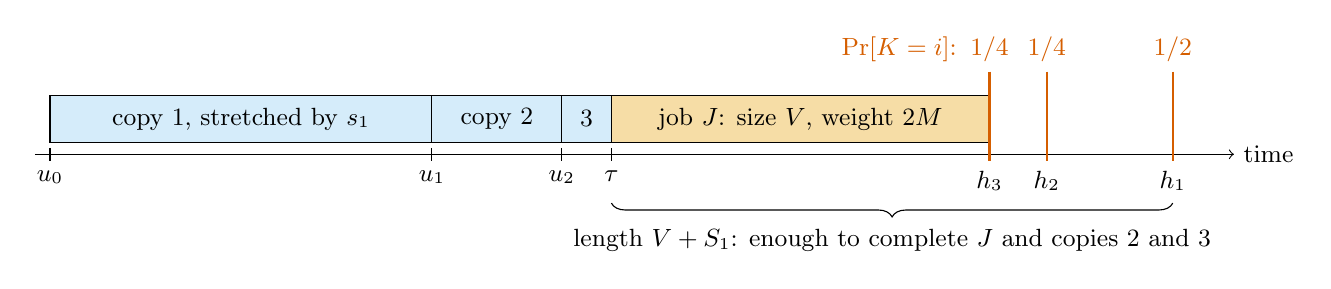
\begin{tikzpicture}[x=0.97cm,y=1cm,font=\small]
    \def\ua{0} \def\ub{5.0} \def\uc{6.7} \def\ud{7.35}
    \def\hc{12.3} \def\hb{13.05} \def\ha{14.7}
    \draw[->] (-0.2,0) -- (15.5,0) node[right] {time};
    \foreach \x/\y/\l in {\ua/\ub/{copy~$1$, stretched by $s_1$},\ub/\uc/{copy~$2$},\uc/\ud/{$3$}} {
      \filldraw[fill=col1!25,draw=black] (\x,0.15) rectangle (\y,0.75);
      \node at ({(\x+\y)/2},0.45) {\l};
    }
    \filldraw[fill=col2!35,draw=black] (\ud,0.15) rectangle (\hc,0.75);
    \node at ({(\ud+\hc)/2},0.45) {job $J$: size $V$, weight $2M$};
    \foreach \x/\l in {\ua/u_0,\ub/u_1,\uc/u_2,\ud/\tau} {
      \draw (\x,0.08) -- (\x,-0.08) node[below] {$\l$};
    }
    \foreach \x/\l/\p in {\hc/h_3/{1/4},\hb/h_2/{1/4},\ha/h_1/{1/2}} {
      \draw[col5,thick] (\x,1.05) -- (\x,-0.08) node[below,black] {$\l$};
      \node[above,col5] at (\x,1.05) {$\p$};
    }
    \node[anchor=south east,col5] at (\hc-0.3,1.05) {$\Pr[K=i]$:};
    \draw[decorate,decoration={brace,amplitude=5pt,mirror}] (\ud,-0.62) -- (\ha,-0.62)
      node[midway,below=6pt] {length $V+S_1$: enough to complete $J$ and copies $2$ and $3$};
  \end{tikzpicture}
  \caption{The amplification step for $k=3$ copies (not to scale). Copy~$i$ is a sample of the hard terminal distribution, stretched in time and size by the factor~$s_i$, which exceeds twice the total length and size of the later copies. The heavy job~$J$ is released at the end~$\tau$ of the last copy. The terminal time is the checkpoint~$h_K$, where $K=i$ with the probability shown above~$h_i$. At checkpoint~$h_i$, there is just enough time to complete~$J$ and copies $i+1,\dots,k$.}
  \label{fig:amplification}
\end{figure}

\paragraph{Amplification.}
Take $k=2M+1$ copies and, immediately after them, release a heavy job~$J$ of weight~$2M$ whose size~$V$ is at least the total size of all copies. The terminal time is one of $k$ checkpoints $h_k<h_{k-1}<\dots<h_1$ after the release of~$J$, where checkpoint~$h_i$ leaves just enough time to complete $J$ and copies $i+1,\dots,k$. We choose the checkpoint~$h_K$ at random, with $\Pr[K\ge i]=2^{1-i}$. At checkpoint~$h_i$, an optimal schedule may complete~$J$ and copies $i+1,\dots,k$, which leaves expected weight at most~$i$ unfinished. At the earliest checkpoint~$h_k$, it may instead complete all copies and leave only~$J$, of weight $k-1$, unfinished. Hence $\E[U^*]\le\E[K]-\Pr[K=k]$.

The algorithm, which does not know~$K$, faces a dilemma at every checkpoint~$h_i$: either $J$ belongs to its robust backlog, or the algorithm has spent almost all the time since the release of~$J$ on~$J$, and then the robust backlogs of copies $1,\dots,i$ are still there. Let~$\ell$ be the smallest index for which $J$ still has remaining size at least~$1$ at~$h_\ell$; since checkpoints with a larger index are earlier, this holds exactly at the checkpoints $h_\ell,\dots,h_k$. At the terminal time~$h_K$, the robust backlog of the algorithm contains the backlogs of all copies $j\le K$ with $j<\ell$, and it contains~$J$ if $K\ge\ell$. Compared with keeping the backlogs $X_1,\dots,X_K$ of all copies, the algorithm may save the copies $\ell,\dots,K$, but $J$ pays for them: conditioned on $K\ge\ell$, the expected number of indices in $\{\ell,\dots,K\}$ is at most two, as $K$ is geometric, and each~$X_j$ is at most~$M$, because of the cap. Thus the algorithm keeps an expected weight of at least $c\,\E[K]$. After normalizing the weights, the gap improves by the factor $\E[K]/(\E[K]-\Pr[K=k])=1+\eta$, where $\eta=1/(2^k-2)$ (\cref{lem:amplification}).

\paragraph{Averaging.}
Amplification improves the gap from~$c$ to $(1+\eta)c$, but the capped robust backlog of the new distribution may be as large as $(k+1)M$. Since~$\eta$ decreases exponentially with the cap, we have to bring the cap down before we amplify again. To this end, we concatenate $m$ copies of a $(c,M)$-hard distribution, take the end of the last copy as the terminal time, and divide all weights by~$m$. The capped backlogs $X_1,\dots,X_m$ of the copies are not independent, because the algorithm adapts to the past, but they are bounded by~$M$ and have conditional expectations at least~$c$. A second-moment bound for the associated martingale shows that their average, capped at~$c$, is still at least $c-\eps$ in expectation (\cref{lem:averaging}). In other words, averaging makes the guarantee almost deterministic.

\paragraph{Putting things together.}
We fix $M\ge4R$ and alternate amplification and averaging. Each round multiplies the gap by $1+\eta/2$ and keeps the cap at~$M$, so after $2^{O(R)}$ rounds the gap exceeds~$2R$ (\cref{thm:hard}). Each round concatenates $2^{O(R)}$ copies, which leads to the weight and size ratios in \cref{thm:quant}.

The idea of improving a lower bound for weighted flow time step by step goes back to Bansal and Chan~\cite{BansalC09}. The new ingredients are an amplification step that does not need to observe the algorithm, because it randomizes the terminal time, and the averaging step, which makes amplification repeatable although its guarantee holds only in expectation.

\subsection{Further related work}

Without weights, randomization does not help on identical parallel machines: the Shortest Remaining Processing Time rule is $O(\log\min\{P,n/m\})$-competitive on $m$ machines, which is best possible also for randomized algorithms~\cite{LeonardiR07}. With weights, Chekuri, Khanna, and Zhu~\cite{ChekuriKZ01} showed that no randomized online algorithm is $O(1)$-competitive on $m\ge2$ identical machines, by a lower bound of $\Omega(\min\{\sqrt P,\sqrt W,(n/m)^{1/4}\})$; our result extends this impossibility to a single machine. Related models include weighted flow time with speed augmentation~\cite{BecchettiLMP01,AnandGK12} and flow time with uncertain job sizes~\cite{AzarLT21,AzarLT22}.

\paragraph{Organization.}
\Cref{sec:prelim} introduces the model and Yao's principle. \Cref{sec:hard} defines hard terminal distributions and shows that they imply \cref{thm:main}. \Cref{sec:construction} constructs hard terminal distributions, and \cref{sec:quantitative} analyzes the weight and size ratios of the construction.

\section{Preliminaries}\label{sec:prelim}

\paragraph{Instances and schedules.}
An \emph{instance}~$I$ is a finite set of jobs; each job $j\in I$ has a release time $r_j\ge0$, a size $p_j>0$, and a weight $w_j>0$. We identify a job with the triple $(r_j,p_j,w_j)$, so an algorithm sees nothing about a job but these parameters; in all instances that we construct, distinct jobs have distinct release times. For a set~$E$ of jobs, we write $w(E)=\sum_{j\in E}w_j$ and $p(E)=\sum_{j\in E}p_j$. A \emph{schedule} of~$I$ assigns to each job $j\in I$ a measurable rate function $x_j\colon[0,\infty)\to[0,1]$ such that $x_j(t)=0$ for $t<r_j$, $\sum_{j\in I}x_j(t)\le1$ for all~$t$, and $\int_0^\infty x_j(t)\dd t\le p_j$. The \emph{remaining size} of~$j$ at time~$t$ is $p_j-\int_0^t x_j(t')\dd t'$; it is continuous and non-increasing in~$t$. Job~$j$ \emph{completes} at the first time~$C_j$ at which its remaining size is zero ($C_j=\infty$ if there is no such time), and it is \emph{unfinished} at time~$t$ if $r_j\le t<C_j$. The weighted flow time of the schedule is
\[
  \sum_{j\in I}w_j(C_j-r_j)=\int_0^\infty U(t)\dd t,
\]
where $U(t)$ denotes the total weight of the jobs that are unfinished at time~$t$. We denote by $\OPT(I)$ the infimum of the weighted flow time over all schedules of~$I$.

Schedules with rates in $\{0,1\}$ are the usual preemptive schedules. Allowing fractional rates does not change the optimum: the preemptive Earliest Deadline First rule, with the completion times of a given schedule as deadlines, completes every job no later than this schedule. For online algorithms, fractional rates only strengthen our lower bounds.

\paragraph{Online algorithms.}
A \emph{deterministic online algorithm}~$A$ maps every instance~$I$ to a schedule $A(I)$ of~$I$ subject to the following non-anticipation condition: for every $t\ge0$ and all instances $I$ and $I'$ that contain the same jobs with release times before~$t$, the schedules $A(I)$ and $A(I')$ assign the same rates to these jobs during $[0,t)$. In other words, the decisions of~$A$ up to time~$t$ depend only on the jobs released before~$t$, including their sizes and weights. In particular, these jobs have the same remaining sizes at time~$t$ in $A(I)$ and in $A(I')$. We write $F_A(I)$ for the weighted flow time of $A(I)$.

A \emph{randomized online algorithm}~$\cA$ is a probability distribution over deterministic online algorithms such that $F_A(I)$ is a random variable for every instance~$I$ when $A\sim\cA$. It is \emph{$R$-competitive} (against an oblivious adversary) if there is a constant~$\Gamma$ such that $\E_{A\sim\cA}[F_A(I)]\le R\cdot\OPT(I)+\Gamma$ for every instance~$I$. We use the easy direction of Yao's principle~\cite{Yao77}; see also~\cite{BorodinE98}.

\begin{lemma}[Yao's principle]\label{lem:yao}
Let $\cD$ be a probability distribution over finitely many instances, and let $R>0$ and $\gamma\in\RR$ be such that every deterministic online algorithm~$A$ satisfies $\E_{I\sim\cD}[F_A(I)]\ge R\cdot\E_{I\sim\cD}[\OPT(I)]+\gamma$. Then for every randomized online algorithm~$\cA$, there is an instance~$I$ in the support of~$\cD$ with $\E_{A\sim\cA}[F_A(I)]\ge R\cdot\OPT(I)+\gamma$.
\end{lemma}

\begin{proof}
If $\E_{A\sim\cA}[F_A(I)]=\infty$ for some~$I$ in the support of~$\cD$, this instance satisfies the claim. Otherwise, taking the expectation of the assumption over $A\sim\cA$ and using linearity of expectation over the finitely many instances in the support of~$\cD$, we obtain
\[
  \E_{I\sim\cD}\bigl[\E_{A\sim\cA}[F_A(I)]-R\cdot\OPT(I)\bigr]\ge\gamma.
\]
Hence some instance in the support of~$\cD$ satisfies the claim.
\end{proof}

\section{Hard terminal distributions}\label{sec:hard}

In this section, we introduce the notion of hardness that underlies our construction, show that it implies lower bounds for weighted flow time, and derive \cref{thm:main} from the existence of hard terminal distributions, which we prove in \cref{sec:construction}.

\paragraph{Terminal distributions.}
A \emph{terminal instance} is a pair $(I,T)$ of an instance~$I$ and a \emph{terminal time} $T>0$ such that all jobs of~$I$ are released before~$T$. A \emph{terminal distribution} is a probability distribution over finitely many terminal instances. An online algorithm processes only the instance~$I$; in particular, the schedule $A(I)$ does not depend on~$T$. In general, $I$ and~$T$ are correlated, so the algorithm may learn something about~$T$ from the jobs it sees, and it may know the distribution in advance.

For a terminal instance $(I,T)$, let $U^*(I,T)$ be the minimum total weight of the jobs that a schedule of~$I$ leaves unfinished at time~$T$; the minimum exists because there are only finitely many sets of jobs. For a deterministic online algorithm~$A$, the \emph{robust backlog} of~$A$ at time~$T$ is the set of jobs of~$I$ whose remaining size in $A(I)$ at time~$T$ is at least~$1$. These jobs are unfinished at time~$T$, and none of them can be completed before time~$T+1$. For $M>0$, the \emph{capped robust backlog} is
\[
  \Phi_M(A;I,T)=\min\bigl\{M,\,w(\text{robust backlog of $A$ at time $T$})\bigr\}.
\]

\begin{definition}\label{def:hard}
Let $0<c\le M$. A terminal distribution~$\cD$ is \emph{$(c,M)$-hard} if
\[
  \E\bigl[U^*(I,T)\bigr]\le1
  \qquad\text{and}\qquad
  \E\bigl[\Phi_M(A;I,T)\bigr]\ge c\quad\text{for every deterministic online algorithm~$A$,}
\]
where the expectations are over $(I,T)\sim\cD$. We call~$c$ the \emph{gap} and~$M$ the \emph{cap}.
\end{definition}

The cap is essential for amplification (\cref{sec:amplification}): it prevents a few copies with a very large backlog from dominating the analysis.

\begin{observation}\label{obs:basic}
\leavevmode
\begin{enumerate}[(a)]
\item\label{obs:base} The terminal distribution that consists of a single job with release time~$0$, size~$2$, and weight~$1$, together with the terminal time~$1$, is $(1,M)$-hard for every $M\ge1$.
\item\label{obs:monotone} If~$\cD$ is $(c,M)$-hard, then~$\cD$ is $(c',M')$-hard for all $0<c'\le c$ and $M'\ge M$.
\item\label{obs:scaling} Let $\lambda>0$ and $0<c\le M$, and let~$\cD$ be a terminal distribution such that $\E[U^*(I,T)]\le\lambda$ and $\E[\Phi_{\lambda M}(A;I,T)]\ge\lambda c$ for every deterministic online algorithm~$A$. Then the terminal distribution obtained from~$\cD$ by dividing all weights by~$\lambda$ is $(c,M)$-hard.
\end{enumerate}
\end{observation}

\begin{proof}
\ref{obs:base}~No schedule completes the job by time~$1$, and in every schedule its remaining size at time~$1$ is at least~$1$. Hence $U^*=1$ and $\Phi_M=\min\{M,1\}=1$.

\ref{obs:monotone}~This follows from $\Phi_{M'}\ge\Phi_M$.

\ref{obs:scaling}~Dividing all weights by~$\lambda$ divides $U^*(I,T)$ by~$\lambda$. For an instance~$I$, let $I/\lambda$ denote the instance with all weights divided by~$\lambda$. Let~$A$ be a deterministic online algorithm, and let~$A_\lambda$ be the algorithm that on input~$I$ runs~$A$ on $I/\lambda$ and uses the same rates, that is, $A_\lambda(I)=A(I/\lambda)$. Since $I$ and $I/\lambda$ have the same release times, $A_\lambda$ satisfies the non-anticipation condition. Both schedules have the same robust backlog, so $\Phi_M(A;I/\lambda,T)=\Phi_{\lambda M}(A_\lambda;I,T)/\lambda$, whose expectation is at least~$c$ by assumption.
\end{proof}

Part~\ref{obs:scaling} uses a simulation because we cannot assume that an algorithm treats $I$ and $I/\lambda$ alike.

\paragraph{From terminal gaps to flow time.}
The following lemma turns a gap in unfinished weight at a single time into a gap in weighted flow time.

\begin{lemma}[Flooding]\label{lem:flooding}
Let $R\ge1$, and let~$\cD$ be a $(2R,M)$-hard terminal distribution. Then for every $\gamma\ge0$, there is a probability distribution~$\hat\cD$ over finitely many instances such that every deterministic online algorithm~$A$ satisfies
\[
  \E_{\hat I\sim\hat\cD}\bigl[F_A(\hat I)\bigr]\ge R\cdot\E_{\hat I\sim\hat\cD}\bigl[\OPT(\hat I)\bigr]+\gamma.
\]
\end{lemma}

\begin{proof}
Let $H\ge1$ and $Q>0$ be such that $T\le H$, $p(I)\le H$, and $w(I)\le Q$ for every terminal instance $(I,T)$ in the support of~$\cD$. Let $d=1/(2M)$, let $n$ be a positive integer, and let $L=nd$. Given $(I,T)\sim\cD$, the instance~$\hat I$ consists of the jobs of~$I$, which we call \emph{old}, and of $n$ \emph{stream} jobs of size~$d$ and weight~$1/2$, released at times $T,T+d,\dots,T+(n-1)d$. Let~$\hat\cD$ be the distribution of~$\hat I$.

\emph{Online cost.} Fix a deterministic online algorithm~$A$ and a terminal instance $(I,T)$ in the support of~$\cD$. As all stream jobs are released at time~$T$ or later, $A(\hat I)$ and $A(I)$ assign the same rates to the old jobs during $[0,T)$, so the old jobs with remaining size at least~$1$ at time~$T$ in $A(\hat I)$ form the robust backlog of~$A$ on $(I,T)$. Let $\Phi=\Phi_M(A;I,T)\le M$. For $0\le\theta<L$, let~$y$ be the total processing that the old jobs receive during $[T,T+\theta)$ in $A(\hat I)$. If $y<1$, then all jobs of the robust backlog are still unfinished at time $T+\theta$, and their total weight is at least~$\Phi$. If $y\ge1$, consider the stream jobs released by time $T+\theta$. Their total size $d\,(\lfloor\theta/d\rfloor+1)$ exceeds~$\theta$, and they received at most $\theta-y$ processing, so their total remaining size exceeds~$y$. As each stream job has size~$d$, more than $y/d$ of them are unfinished at time~$T+\theta$, and their total weight exceeds $y/(2d)=My\ge M\ge\Phi$. In both cases, the total weight of the jobs unfinished at time $T+\theta$ is at least~$\Phi$. Integrating over $\theta\in[0,L)$ yields $F_A(\hat I)\ge L\cdot\Phi$, and by the hardness of~$\cD$,
\[
  \E\bigl[F_A(\hat I)\bigr]\ge L\cdot\E[\Phi]\ge 2RL.
\]

\emph{Optimal cost.} Consider the following schedule of~$\hat I$. Until time~$T$, follow a schedule of~$I$ that leaves weight $U^*(I,T)$ unfinished at time~$T$. During $[T,T+L)$, process each stream job in the $d$ time units after its release. After time $T+L$, complete the remaining old jobs. The old jobs contribute at most~$QH$ to the weighted flow time before time~$T$, exactly $U^*(I,T)\cdot L$ during $[T,T+L)$, and at most~$QH$ afterwards, since their total remaining size is at most~$H$. The stream jobs contribute $n\cdot d/2=L/2$. Hence $\OPT(\hat I)\le 2QH+(U^*(I,T)+1/2)\,L$, and therefore
\[
  \E\bigl[\OPT(\hat I)\bigr]\le 2QH+\tfrac32L.
\]

Combining both bounds, $\E[F_A(\hat I)]-R\cdot\E[\OPT(\hat I)]\ge R\,(L/2-2QH)$, which is at least~$\gamma$ if~$n$ is large enough. Since the choice of~$n$ does not depend on~$A$, this proves the lemma.
\end{proof}

The main technical result is the existence of hard terminal distributions with arbitrarily large gaps.

\begin{theorem}\label{thm:hard}
For every $R\ge1$, there is a $(2R,M)$-hard terminal distribution with $M=\lceil4R\rceil$.
\end{theorem}

\begin{proof}[Proof of \cref{thm:main}]
Let $R\ge1$ and $\gamma\ge0$. By \cref{thm:hard} and \cref{lem:flooding}, there is a distribution~$\hat\cD$ over finitely many instances such that every deterministic online algorithm~$A$ satisfies $\E[F_A(\hat I)]\ge R\cdot\E[\OPT(\hat I)]+\gamma$. This is the second statement. For the first one, let~$\cA$ be a randomized online algorithm and $\Gamma\ge0$. Applying \cref{lem:yao} to the distribution~$\hat\cD$ obtained for $\gamma=\Gamma+1$ yields an instance~$\hat I$ with $\E_{A\sim\cA}[F_A(\hat I)]\ge R\cdot\OPT(\hat I)+\Gamma+1$, so~$\cA$ is not $R$-competitive with additive constant~$\Gamma$. Since $R$ and~$\Gamma$ are arbitrary, no randomized online algorithm is $O(1)$-competitive.
\end{proof}

\section{Constructing hard terminal distributions}\label{sec:construction}

We prove \cref{thm:hard} by alternating two operations on hard terminal distributions. Amplification (\cref{sec:amplification}) multiplies the gap by $1+\eta$ for a small $\eta>0$ that depends on the cap, but it increases the cap. Averaging (\cref{sec:averaging}) reduces the cap to the gap while losing only a little in the gap. Both operations concatenate independent copies of a terminal distribution at decreasing time scales, which we analyze first.

\subsection{Copies at decreasing time scales}\label{sec:copies}

Let~$\cD$ be a terminal distribution, let $H\ge1$ be such that $T\le H$ and $p(I)\le H$ for every $(I,T)$ in the support of~$\cD$, and let~$m$ be a positive integer; we write $[m]=\{1,\dots,m\}$. We set $\rho=2H+1$ and
\[
  S_i=\rho^{m-i}-1\quad\text{for } i\in\{0,\dots,m\},\qquad
  s_i=2\rho^{m-i}\quad\text{for } i\in[m],\qquad
  V=S_0=\rho^m-1.
\]
These numbers satisfy, for every $i\in[m]$,
\begin{equation}\label{eq:scales}
  S_i=H\sum_{j=i+1}^m s_j
  \qquad\text{and}\qquad
  s_i-S_i=S_i+2,
\end{equation}
where the first identity is a geometric sum; it also holds for $i=0$. We draw $(I_1,T_1),\dots,(I_m,T_m)$ independently from~$\cD$, and we let $u_0=0$ and $u_i=u_{i-1}+s_iT_i$ for $i\in[m]$. For every $i\in[m]$, \emph{copy~$i$} contains, for each job $j\in I_i$, a job with release time $u_{i-1}+s_ir_j$, size $s_ip_j$, and weight~$w_j$, which we call the copy of~$j$. Thus copy~$i$ is the instance~$I_i$, stretched in time and size by the factor~$s_i$ and started at time~$u_{i-1}$; its terminal time is~$u_i$. The \emph{concatenation}~$\bar I$ is the union of copies $1,\dots,m$, and $\tau=u_m$ is its \emph{end}. The concatenation depends on the choice of~$H$; everything below holds for every admissible~$H$, and we suppress~$H$ in the notation.

The choice of the scales ensures that all copies after copy~$i$ fit into a time interval of length~$S_i$, while the robust backlog of copy~$i$ survives them with remaining size at least $S_i+2$.

\begin{lemma}\label{lem:copies}
Let~$\cD$ be a $(c,M)$-hard terminal distribution, and let~$\bar I$ be the concatenation of $m$ copies of~$\cD$ with end~$\tau$, as above.
\begin{enumerate}[(i)]
\item\label{it:geometry} The jobs of copy~$i$ are released during $[u_{i-1},u_i)$. For every $i\in\{0,\dots,m\}$, copies $i+1,\dots,m$ have total size at most~$S_i$, and $\tau-u_i\le S_i$. In particular, $p(\bar I)\le V$ and $\tau\le V$.
\item\label{it:offline} There is a schedule of~$\bar I$ in which, for every $i\in[m]$, the jobs of copy~$i$ that are unfinished at time~$\tau$ have total weight $B_i=U^*(I_i,T_i)$. Moreover, $\E[B_i]\le1$.
\item\label{it:online} Let~$A$ be a deterministic online algorithm, and let~$\tilde I$ be an instance that consists of~$\bar I$ and possibly further jobs released at time~$\tau$ or later; these jobs may depend arbitrarily on $(I_1,T_1),\dots,(I_m,T_m)$. For $i\in[m]$, let~$E_i$ be the set of jobs of copy~$i$ whose remaining size at time~$u_i$ in $A(\tilde I)$ is at least~$s_i$, and let $X_i=\min\{M,w(E_i)\}$. Then $X_i$ is determined by $(I_1,T_1),\dots,(I_i,T_i)$, and
\[
  \E\bigl[X_i\bigm|(I_1,T_1),\dots,(I_{i-1},T_{i-1})\bigr]\ge c.
\]
Moreover, every job of~$E_i$ has remaining size at least $S_i+2$ at time~$\tau$.
\end{enumerate}
\end{lemma}

In part~\ref{it:online}, the set~$E_i$ is the robust backlog of copy~$i$ measured in the units of copy~$i$: after shrinking time and sizes by the factor~$s_i$, its jobs have remaining size at least~$1$ at the terminal time of copy~$i$.

\begin{proof}
\ref{it:geometry}~A job of copy~$i$ is released at time $u_{i-1}+s_ir_j$ with $0\le r_j<T_i$, hence during $[u_{i-1},u_i)$. Copy~$i'$ has total size $s_{i'}\,p(I_{i'})\le s_{i'}H$, and it is released during the interval $[u_{i'-1},u_{i'})$ of length $s_{i'}T_{i'}\le s_{i'}H$. Summing over $i'>i$ and using~\eqref{eq:scales} proves the second claim; the case $i=0$ gives the third.

\ref{it:offline}~For $i\in[m]$, fix a schedule of~$I_i$ that leaves weight $U^*(I_i,T_i)$ unfinished at time~$T_i$, with rate functions~$x_j$. During $[u_{i-1},u_i)$, process the copy of each $j\in I_i$ at rate $x_j((t-u_{i-1})/s_i)$ at time~$t$. This stretched schedule processes the copy of~$j$ only after its release, and the copy is unfinished at time~$u_i$ if and only if~$j$ is unfinished at time~$T_i$. Since the intervals $[u_{i-1},u_i)$ are disjoint, these schedules combine into a schedule of~$\bar I$, which does not process copy~$i$ after time~$u_i$. Moreover, $\E[B_i]=\E_{(I,T)\sim\cD}[U^*(I,T)]\le1$.

\ref{it:online}~Fix $i\in[m]$ and condition on $(I_1,T_1),\dots,(I_{i-1},T_{i-1})$; since~$\cD$ has finite support, we condition on an event of positive probability. Then copies $1,\dots,i-1$ and the time~$u_{i-1}$ are fixed. We show that, from the point of view of copy~$i$, the algorithm~$A$ behaves like a deterministic online algorithm~$A_i$ for~$\cD$.

\emph{The algorithm~$A_i$.} For an arbitrary instance~$I$, let $\sigma_i(I)$ be the instance obtained from~$I$ in the same way as copy~$i$ is obtained from~$I_i$, that is, by stretching~$I$ by the factor~$s_i$ and starting it at time~$u_{i-1}$, and let $\bar I_i(I)$ be the union of copies $1,\dots,i-1$ and $\sigma_i(I)$. On input~$I$, the algorithm~$A_i$ runs~$A$ on $\bar I_i(I)$ and processes each job $j\in I$ at time~$t$ at the rate at which~$A$ processes the copy of~$j$ at time $u_{i-1}+s_it$. This is a schedule of~$I$: the rates sum to at most~$1$, job~$j$ is not processed before~$r_j$ because its copy is not processed before $u_{i-1}+s_ir_j$, and job~$j$ receives at most~$p_j$ processing because its copy receives at most~$s_ip_j$. The algorithm~$A_i$ satisfies the non-anticipation condition, because the decisions of~$A$ before time $u_{i-1}+s_it$ depend only on copies $1,\dots,i-1$ and on the copies of the jobs of~$I$ released before~$t$. Since time is stretched by the factor~$s_i$, the remaining size of~$j$ at time~$t$ in $A_i(I)$ equals $1/s_i$ times the remaining size of the copy of~$j$ at time $u_{i-1}+s_it$ in $A(\bar I_i(I))$.

\emph{Agreement before~$u_i$.} The instances $\bar I_i(I_i)$ and~$\tilde I$ contain the same jobs with release times before~$u_i$: copies $1,\dots,i$ are released before~$u_i$ by~\ref{it:geometry}, while copies $i+1,\dots,m$ and all further jobs of~$\tilde I$ are released at time~$u_i$ or later. By the non-anticipation condition, $A(\bar I_i(I_i))$ and $A(\tilde I)$ process copies $1,\dots,i$ in the same way during $[0,u_i)$. In particular, $X_i$ is determined by $(I_1,T_1),\dots,(I_i,T_i)$. Moreover, as $u_i=u_{i-1}+s_iT_i$, a job of copy~$i$ belongs to~$E_i$ if and only if its original has remaining size at least~$1$ at time~$T_i$ in $A_i(I_i)$. Hence
\[
  X_i=\Phi_M(A_i;I_i,T_i).
\]
The algorithm~$A_i$ depends only on the event we condition on, while $(I_i,T_i)$ is independent of this event and distributed according to~$\cD$. Since~$\cD$ is $(c,M)$-hard, the conditional expectation of~$X_i$ is at least~$c$.

\emph{Survival.} A job of~$E_i$ has remaining size at least~$s_i$ at time~$u_i$ and receives at most $\tau-u_i\le S_i$ processing during $[u_i,\tau)$. By~\eqref{eq:scales}, its remaining size at time~$\tau$ is at least $s_i-S_i=S_i+2$.
\end{proof}

\subsection{Amplification}\label{sec:amplification}

Let $M\ge1$ be an integer and $k=2M+1$. Let~$\cD$ be a terminal distribution with a bound~$H$ as in \cref{sec:copies}, and let~$\bar I$ be the concatenation of~$k$ copies of~$\cD$, with the notation of \cref{sec:copies} for $m=k$. We add a job~$J$ with release time~$\tau$, size~$V$, and weight~$2M$, and we define the \emph{checkpoints}
\[
  h_i=\tau+V+S_i\qquad(i\in[k]).
\]
Since $S_1>S_2>\dots>S_k=0$, we have $h_1>h_2>\dots>h_k=\tau+V$; a larger index means an earlier checkpoint. Independently of the copies, we draw $K\in[k]$ with $\Pr[K\ge i]=2^{1-i}$ for all $i\in[k]$; for instance, $K$ is the number of fair coin flips up to and including the first head, truncated at~$k$. Note that $\E[K]=\sum_{i=1}^k\Pr[K\ge i]=2-2^{1-k}$ and $\Pr[K=k]=2^{1-k}$, and let
\[
  \beta=\E[K]-\Pr[K=k]=2-2^{2-k}.
\]
The \emph{amplified} terminal distribution $\Amp_M(\cD)$ is the distribution of the terminal instance $(\bar I\cup\{J\},h_K)$ with all weights divided by~$\beta$.

\begin{lemma}\label{lem:amplification}
Let $M\ge1$ be an integer, $k=2M+1$, and $\eta=1/(2^k-2)$. If~$\cD$ is $(c,M)$-hard, then $\Amp_M(\cD)$ is $((1+\eta)c,(k+1)M)$-hard.
\end{lemma}

\begin{proof}
All jobs of $\bar I\cup\{J\}$ are released by time $\tau<h_K$, and the support is finite, so $\Amp_M(\cD)$ is a terminal distribution. We show that the terminal instance $(\bar I\cup\{J\},h_K)$, before the weights are divided by~$\beta$, satisfies
\begin{equation}\label{eq:amp-goal}
  \E\bigl[U^*(\bar I\cup\{J\},h_K)\bigr]\le\beta
  \qquad\text{and}\qquad
  \E\bigl[\Phi_{(k+1)M}(A;\bar I\cup\{J\},h_K)\bigr]\ge c\,\E[K]
\end{equation}
for every deterministic online algorithm~$A$. This implies the lemma by \cref{obs:basic}\ref{obs:scaling} with $\lambda=\beta$, because $\Phi_{\beta(k+1)M}\ge\Phi_{(k+1)M}$ (as $\beta\ge1$), $(1+\eta)c\le2M\le(k+1)M$, and
\[
  \frac{\E[K]}{\beta}=\frac{2-2^{1-k}}{2-2^{2-k}}=\frac{2^k-1}{2^k-2}=1+\eta.
\]

\emph{Offline.} Follow the schedule of \cref{lem:copies}\ref{it:offline} until time~$\tau$. If $K=i<k$, use the interval $[\tau,h_i)$ of length $V+S_i$ to complete~$J$, of size~$V$, and the remaining jobs of copies $i+1,\dots,k$, of total size at most~$S_i$ by \cref{lem:copies}\ref{it:geometry}. Then only jobs of copies $1,\dots,i$ are unfinished at time~$h_i$, and their total weight is at most $B_1+\dots+B_i$. If $K=k$, use the interval $[\tau,\tau+V)$ to complete all remaining jobs of~$\bar I$, whose total size is at most $p(\bar I)\le V$. Then only~$J$ is unfinished at time~$h_k$, and its weight is $2M=k-1$. Write $U^*=U^*(\bar I\cup\{J\},h_K)$. Since~$K$ is independent of the copies and $\E[B_j]\le1$ for all~$j$, we obtain $\E[U^*\mid K=i]\le i$ for $i<k$ and $\E[U^*\mid K=k]\le k-1$. Hence $\E[U^*]\le\E[K]-\Pr[K=k]=\beta$.

\emph{Online.} Fix a deterministic online algorithm~$A$ and the copies $(I_1,T_1),\dots,(I_k,T_k)$; we first take the expectation over~$K$ only. The variable~$K$ affects the terminal time but not the instance, so the schedule $A(\bar I\cup\{J\})$ is fixed. Let~$E_j$ and~$X_j$ be as in \cref{lem:copies}\ref{it:online} for $\tilde I=\bar I\cup\{J\}$. Let~$\ell$ be the smallest $i\in[k]$ such that~$J$ has remaining size at least~$1$ at time~$h_i$, and let $\ell=k+1$ if there is no such~$i$. Since remaining sizes do not increase over time and checkpoints with a larger index are earlier, $J$ has remaining size at least~$1$ at time~$h_i$ if and only if $i\ge\ell$.

We claim that for all $j<\ell$ and all $i\ge j$, every job of~$E_j$ has remaining size at least~$1$ at time~$h_i$. As $h_i\le h_j$, it suffices to consider $i=j$. Because $j<\ell$, job~$J$ has remaining size less than~$1$ at time~$h_j$, so it received more than $V-1$ processing during $[\tau,h_j)$. This leaves less than $(h_j-\tau)-(V-1)=S_j+1$ processing for all other jobs during this interval. By \cref{lem:copies}\ref{it:online}, every job of~$E_j$ has remaining size at least $S_j+2$ at time~$\tau$, and hence more than~$1$ at time~$h_j$.

By the claim, the robust backlog of~$A$ at time~$h_K$ contains~$E_j$ for all $j\le K$ with $j<\ell$, and it contains~$J$ if $K\ge\ell$. These sets are pairwise disjoint and $w(E_j)\ge X_j$, so the weight of the robust backlog is at least
\[
  Z=\sum_{j\le K,\;j<\ell}X_j+2M\cdot\bone[K\ge\ell].
\]
Moreover, $Z\le(k+1)M$: if $K<\ell$, then~$Z$ is a sum of at most~$k$ terms~$X_j\le M$, and if $K\ge\ell$, then~$Z$ is a sum of at most~$k-1$ such terms and~$2M$. Hence $\Phi_{(k+1)M}(A;\bar I\cup\{J\},h_K)\ge Z$. Taking the expectation over~$K$, with~$\ell$ and all~$X_j$ fixed, we obtain
\[
  \E_K[Z]=\sum_{j<\ell}\Pr[K\ge j]\,X_j+2M\cdot\Pr[K\ge\ell]\ge\sum_{j=1}^k\Pr[K\ge j]\,X_j,
\]
where the inequality uses $X_j\le M$ and the geometric tail bound $\sum_{j=\ell}^k\Pr[K\ge j]\le2\Pr[K\ge\ell]$. For $\ell=k+1$, both sides of this bound vanish, and for $\ell\le k$,
\[
  \sum_{j=\ell}^k\Pr[K\ge j]=\sum_{j=\ell}^k2^{1-j}<2\cdot2^{1-\ell}=2\Pr[K\ge\ell].
\] This is the step in which~$J$ pays for the copies $\ell,\dots,K$ that the algorithm may have cleared. Finally, taking the expectation over the copies and using $\E[X_j]\ge c$ from \cref{lem:copies}\ref{it:online}, we obtain
\[
  \E\bigl[\Phi_{(k+1)M}(A;\bar I\cup\{J\},h_K)\bigr]\ge\E[Z]\ge c\sum_{j=1}^k\Pr[K\ge j]=c\,\E[K].
\]
This proves~\eqref{eq:amp-goal} and the lemma.
\end{proof}

For example, let $M=1$ and let~$\cD$ be the $(1,1)$-hard single-job distribution of \cref{obs:basic}\ref{obs:base}. Then $k=3$, every algorithm has an expected robust backlog of at least $\E[K]=7/4$ at the terminal time, an optimal schedule leaves expected weight at most $\beta=3/2$ unfinished, and the gap after normalization is~$7/6$. One can check that both bounds are tight in this example.

\subsection{Averaging}\label{sec:averaging}

For a terminal distribution~$\cD$ with a bound~$H$ as in \cref{sec:copies} and a positive integer~$m$, the \emph{averaged} terminal distribution $\Avg_m(\cD)$ is the distribution of the terminal instance $(\bar I,\tau)$, where~$\bar I$ is the concatenation of~$m$ copies of~$\cD$ and~$\tau$ is its end, with all weights divided by~$m$.

\begin{lemma}\label{lem:averaging}
Let~$\cD$ be a $(c,M)$-hard terminal distribution, let $0<\eps<c$, and let $m=\lceil(M/\eps)^2\rceil$. Then $\Avg_m(\cD)$ is $(c-\eps,c)$-hard.
\end{lemma}

\begin{proof}
By \cref{lem:copies}\ref{it:geometry}, all jobs of~$\bar I$ are released before $u_m=\tau$, so $\Avg_m(\cD)$ is a terminal distribution. By \cref{obs:basic}\ref{obs:scaling} with $\lambda=m$, it suffices to show that $\E[U^*(\bar I,\tau)]\le m$ and $\E[\Phi_{cm}(A;\bar I,\tau)]\ge(c-\eps)\,m$ for every deterministic online algorithm~$A$, where the weights are not divided by~$m$. The first bound follows from \cref{lem:copies}\ref{it:offline}, since $U^*(\bar I,\tau)\le B_1+\dots+B_m$.

Fix~$A$, and let~$E_i$ and~$X_i$ be as in \cref{lem:copies}\ref{it:online} for $\tilde I=\bar I$. Every job of~$E_i$ has remaining size at least $S_i+2\ge2$ at time~$\tau$, so the robust backlog of~$A$ at time~$\tau$ contains the pairwise disjoint sets $E_1,\dots,E_m$, and
\[
  \Phi_{cm}(A;\bar I,\tau)\ge\min\{cm,Y\},\qquad\text{where}\qquad Y=\sum_{i=1}^mX_i.
\]
Let~$\cF_i$ be the $\sigma$-algebra generated by $(I_1,T_1),\dots,(I_i,T_i)$, let $\mu_i=\E[X_i\mid\cF_{i-1}]$, and let $\Delta=\sum_{i=1}^m(X_i-\mu_i)$. By \cref{lem:copies}\ref{it:online}, $\mu_i\ge c$, so $Y\ge cm+\Delta$. The variables~$X_i$ need not be independent, since the algorithm adapts to the past, but the differences $X_i-\mu_i$ form a martingale difference sequence: $X_i-\mu_i$ is $\cF_i$-measurable, $\E[X_i-\mu_i\mid\cF_{i-1}]=0$, and $|X_i-\mu_i|\le M$ because $X_i$ and~$\mu_i$ lie in $[0,M]$. For $i<j$, conditioning on~$\cF_{j-1}$ shows $\E[(X_i-\mu_i)(X_j-\mu_j)]=0$, so $\E[\Delta^2]=\sum_{i=1}^m\E[(X_i-\mu_i)^2]\le mM^2$. Using $(cm-Y)^+\le(-\Delta)^+\le|\Delta|$ and the Cauchy--Schwarz inequality, we conclude
\[
  \E\bigl[\min\{cm,Y\}\bigr]=cm-\E\bigl[(cm-Y)^+\bigr]\ge cm-\E\bigl[|\Delta|\bigr]\ge cm-\sqrt{\E[\Delta^2]}\ge cm-M\sqrt m\ge(c-\eps)\,m,
\]
where the last inequality uses $m\ge(M/\eps)^2$.
\end{proof}

\subsection{Proof of \texorpdfstring{\cref{thm:hard}}{Theorem 3.4}}\label{sec:iteration}

Let $R\ge1$, and let
\[
  M=\lceil4R\rceil,\qquad k=2M+1,\qquad \eta=\frac1{2^k-2},\qquad m=\biggl\lceil\Bigl(\frac{2(k+1)M}{\eta}\Bigr)^2\biggr\rceil.
\]
Let~$\cD_0$ be the $(1,M)$-hard terminal distribution of \cref{obs:basic}\ref{obs:base}, and for $q\ge1$, let $\cD_q=\Avg_m(\Amp_M(\cD_{q-1}))$, where both operations may use any bound~$H$ as in \cref{sec:copies}; the specific choice matters only in \cref{sec:quantitative}. We call the step from~$\cD_{q-1}$ to~$\cD_q$ the $q$-th \emph{round}. Let $c_q=(1+\eta/2)^q$, and let~$N$ be the smallest integer with $c_N\ge2R$.

We show by induction that~$\cD_q$ is $(c_q,M)$-hard for $q=0,\dots,N$. The case $q=0$ holds. Let $1\le q\le N$, and assume that~$\cD_{q-1}$ is $(c_{q-1},M)$-hard. By \cref{lem:amplification}, $\Amp_M(\cD_{q-1})$ is $((1+\eta)c_{q-1},(k+1)M)$-hard. We apply \cref{lem:averaging} with $\eps=\eta/2<(1+\eta)c_{q-1}$, for which the number of copies is $\lceil((k+1)M/\eps)^2\rceil=m$. Hence~$\cD_q$ is $((1+\eta)c_{q-1}-\eta/2,\,(1+\eta)c_{q-1})$-hard. Since $c_{q-1}\ge1$, we have $(1+\eta)c_{q-1}-\eta/2\ge(1+\eta/2)c_{q-1}=c_q$. Since $q-1<N$, we have $c_{q-1}<2R$, and as $\eta<1$, the cap satisfies $(1+\eta)c_{q-1}<4R\le M$. By \cref{obs:basic}\ref{obs:monotone}, $\cD_q$ is $(c_q,M)$-hard.

In particular, $\cD_N$ is $(c_N,M)$-hard and hence $(2R,M)$-hard by \cref{obs:basic}\ref{obs:monotone}. This proves \cref{thm:hard}.

By induction on~$q$, all instances in the support of~$\cD_q$ have the same number of jobs, and flooding (\cref{lem:flooding}) adds the same number of jobs to each instance. Hence our lower bounds hold even for algorithms that know the number of jobs in advance.

\section{Dependence on the weight and size ratios}\label{sec:quantitative}

For an instance~$I$, let $W(I)=\max_{j\in I}w_j/\min_{j\in I}w_j$ and $P(I)=\max_{j\in I}p_j/\min_{j\in I}p_j$. In this section, all logarithms are binary. We analyze the construction of \cref{sec:iteration} and prove the following refinement of \cref{thm:main}.

\begin{theorem}\label{thm:quant-refined}
There is an absolute constant $C\ge1$ such that for all $R\ge1$ and $\gamma\ge0$, there is a probability distribution~$\hat\cD$ over finitely many instances such that every instance~$\hat I$ in its support satisfies
\[
  W(\hat I)\le2^{2^{CR}}\qquad\text{and}\qquad P(\hat I)\le2^{2^{2^{CR}}},
\]
and every deterministic online algorithm~$A$ satisfies $\E[F_A(\hat I)]\ge R\cdot\E[\OPT(\hat I)]+\gamma$.
\end{theorem}

\begin{proof}
Let $M$, $k$, $\eta$, $m$, $N$, and $\cD_0,\dots,\cD_N$ be as in \cref{sec:iteration}, and let $\beta=2-2^{2-k}$ be the normalization factor of amplification. We apply \cref{lem:flooding} to the $(2R,M)$-hard terminal distribution~$\cD_N$, which yields~$\hat\cD$. It remains to bound the weight and size ratios. Recall that the stream jobs have weight~$1/2$ and size $1/(2M)$.

\emph{Weights.} We show by induction that for $q\ge0$, all weights in~$\cD_q$ lie in $[(\beta m)^{-q},1]$. The only weight in~$\cD_0$ is~$1$. Amplification keeps the weights of the copies, adds the weight~$2M$, and divides all weights by~$\beta$; averaging then divides all weights by~$m$. Hence the weights in~$\cD_q$ lie in $[w_{\min}/(\beta m),\,\max\{w_{\max},2M\}/(\beta m)]$, where $w_{\min}$ and~$w_{\max}$ are the smallest and largest weights in~$\cD_{q-1}$. The claim follows because $w_{\max}\le1$ and $2M\le m\le\beta m$. We have $N\ge1$ because $c_0=1<2R$, so $(\beta m)^{-N}\le1/2$, and the stream weight~$1/2$ also lies in $[(\beta m)^{-N},1]$. Thus $W(\hat I)\le(\beta m)^N\le(2m)^N$.

\emph{Sizes.} We fix the bounds used by the construction. Let $H_0=2$, and for $q\ge1$, let
\[
  \hat H_q=3\bigl((2H_{q-1}+1)^k-1\bigr)\qquad\text{and}\qquad H_q=(2\hat H_q+1)^m-1.
\]
In round~$q$, amplification uses the bound~$H_{q-1}$ for~$\cD_{q-1}$, and averaging uses the bound~$\hat H_q$ for $\Amp_M(\cD_{q-1})$. These bounds are valid: $H_0$ bounds the terminal time and the size in~$\cD_0$. If~$H_{q-1}$ bounds the terminal times and total sizes in~$\cD_{q-1}$, then in $\Amp_M(\cD_{q-1})$, the concatenation of~$k$ copies has total size at most $V=(2H_{q-1}+1)^k-1$ by \cref{lem:copies}\ref{it:geometry}, so the total size including~$J$ is at most~$2V$, and the terminal time is at most $h_1=\tau+V+S_1\le3V=\hat H_q$. Applying \cref{lem:copies}\ref{it:geometry} to the $m$ copies of averaging shows that~$H_q$ bounds the terminal times and total sizes in~$\cD_q$. Moreover, all jobs in~$\cD_q$ have size at least~$2$: this holds for~$\cD_0$, copies stretch sizes by factors $s_i\ge2$, and the job~$J$ added by amplification has size $V=\rho^k-1\ge\rho-1=2H_{q-1}\ge2$. Consequently, all sizes in~$\hat I$ lie in $[1/(2M),H_N]$, and $P(\hat I)\le2MH_N$.

To bound~$H_N$, let $G_q=2H_q+1$, so that $G_0=5$ and $G_q\ge5$ for all~$q$. Since $2\hat H_q+1\le6\,G_{q-1}^k$ and $2\cdot6^m\le25^m\le G_{q-1}^{2m}$, we have
\[
  G_q\le2\,(2\hat H_q+1)^m\le2\cdot6^m\,G_{q-1}^{km}\le G_{q-1}^{(k+2)m},
\]
and therefore $\log H_N<\log G_N\le((k+2)m)^N\log5$.

\emph{Growth in~$R$.} We have $M\le5R$ and $k\le11R$. Since $1/\eta<2^k$, we get $\log m\le2k+2\log(2(k+1)M)+1=O(R)$, and since $\ln(1+x)\ge x/2$ for $x\in[0,1]$, the number of rounds satisfies
\[
  N\le1+\frac{\ln(2R)}{\ln(1+\eta/2)}\le1+\frac{4\ln(2R)}{\eta}\le1+2^{k+2}\ln(2R)=2^{O(R)}.
\]
Hence $\log W(\hat I)\le N\log(2m)=2^{O(R)}$. Moreover, using $\log(a+b)\le1+\log a+\log b$ for $a,b\ge1$,
\begin{align*}
  \log\log P(\hat I)
  &\le\log\bigl(\log(2M)+((k+2)m)^N\log5\bigr)\\
  &\le1+\log\log(2M)+N\log((k+2)m)+\log\log5=2^{O(R)}.
\end{align*}
All constants in the $O$-notation are absolute, so there is an absolute constant $C\ge1$ with $\log W(\hat I)\le2^{CR}$ and $\log\log P(\hat I)\le2^{CR}$ for all $R\ge1$.
\end{proof}

\begin{proof}[Proof of \cref{thm:quant}]
Let~$C$ be the constant of \cref{thm:quant-refined}, let~$\cA$ be a randomized online algorithm, and let $R=\min\{\log\log W,\log\log\log P\}/C$. If $R<1$, there is nothing to show, since no algorithm has competitive ratio less than~$1$. Otherwise, let $\Gamma\ge0$. By \cref{thm:quant-refined} with $\gamma=\Gamma+1$ and \cref{lem:yao}, there is an instance~$\hat I$ with $W(\hat I)\le2^{2^{CR}}\le W$ and $P(\hat I)\le2^{2^{2^{CR}}}\le P$ such that $\E_{A\sim\cA}[F_A(\hat I)]\ge R\cdot\OPT(\hat I)+\Gamma+1$. Hence, on instances with weight and size ratios at most~$W$ and~$P$, the algorithm~$\cA$ is not $R$-competitive, and its competitive ratio is at least $R=\Omega(\min\{\log\log W,\log\log\log P\})$.
\end{proof}

\section{Concluding remarks}\label{sec:conclusion}

We have shown that randomization does not allow a constant competitive ratio for online weighted flow time on a single machine. Our lower bound of $\Omega(\min\{\log\log W,\log\log\log P\})$ is exponentially weaker than the deterministic lower bound of Bansal and Chan~\cite{BansalC09}, and the best known upper bound is $O(\log\min\{P,D,W\})$, achieved by a deterministic algorithm~\cite{AzarT18}. The weak dependence on~$W$ and~$P$ stems from the amplification step: its gain $\eta=1/(2^{2M+1}-2)$ is exponentially small in the cap~$M$, so $2^{\Theta(R)}$ rounds are needed to reach the gap~$2R$. An amplification step whose gain is only polynomially small in the cap would lead to lower bounds that are polynomial in $\log W$ and $\log\log P$. More generally, it remains open whether randomized algorithms can beat the deterministic lower bound, for example by achieving a competitive ratio of $O(\log\log W)$.

\printbibliography

\end{document}
